This section provides a conceptual framework for understanding how birth spacing changes
and guiding the subsequent analysis.
In non-Western countries, lower fertility is associated with longer birth spacing, but 
outside a ``natural fertility'' regime it is not clear that lower fertility necessarily 
leads to longer spacing \citet{Newman1988,Rutstein2011,Casterline2016}.
Thus, I first introduce three potential explanations that link fertility and birth 
spacing decisions: economic conditions, desired child outcomes, and son preference 
\citep{Casterline2016,Portner2018}.
Next, I argue that female education and area of residence are the most important factors 
to consider in the empirical analysis and discuss how they tie into the three theories.


The dramatic improvements in economic conditions in India is best illustrated by the 
doubling of real wages between 1987 and 2011 \citep{Klasen2015}.
Economic theory predicts that the effect of higher wages on fertility is determined by 
the relative strengths of the substitution and income effects.
The substitute effect captures that as a good becomes more expensive relative to other
goods, people substitute away from the now more expensive good and towards other goods.
With higher wages, the substitute effect predicts that people work more and spend less 
time on other time-intensive non-wage earning activities, such as children or leisure.
The income effect captures that even if we ignore the substitution effect and hold hours 
worked constant higher wages increase the available income. 
This positive income effect leads people to spend more time on time-intensive activities 
such as children and leisure and less time working.

Empirically, higher female wages generally lowers fertility, whereas higher male 
wages increases fertility \citet{Hotz1997,schultz97}.
This pattern is consistent with women spending substantially more time on child care 
than men, leading to the substitution effect dominating for women while the income
effect dominates for men.

In addition to lowering fertility, higher female wages will tend to shorten spacing between 
children if having children requires the mother to reduce her economic activities.
Specifically, shortening birth spacing allows parents to take advantage of economies of 
scale in childrearing---for example, looking after two children simultaneously requires 
less than double the time needed to look after one child \citep{Vijverberg1982,Hotz1997}.
The reduction in the length of birth intervals from higher female wages will be more 
pronounced the more women participate in the labor force rather than working at home as 
economic activities at home are more compatible with child rearing.

[bla, bla]
The effect of increasing male wages on birth spacing is ambiguous.
On one hand, if fertility increases one might expect spacing to become shorter, although 
unless the updated desired fertility is close to natural fertility the higher desired 
fertility could simply be accommodated by having the last child later in life.
On the other hand, higher income could ``purchase'' both higher fertility and 
better quality children.
If child quality is increasing in birth spacing we would then expect higher male wages
to lead to longer birth spacing.


Parents care not only about how many children they have but also about the outcomes
for the children, and, everything else equal, more children means less resources to invest 
per child.
Hence, with declining fertility we should see better child outcomes such as lower 
mortality and more schooling.
However, with increasing income, it is, in principle, possible to have both more
children and better outcomes for them.
Increasing returns to education might make the parents reduce fertility and invest 
more in each of the children's education \citep{Rosenzweig1982a}.

Longer spacing between births is generally expected to have positive effects on 
child outcomes and if fertility falls because of increased desired for better child
outcomes we would, therefore, also expect spacing to increase.
The clearest example of birth spacing affecting child outcomes is for health,
where very short spacing---approximately 24 months or less---leads to worse health 
and mortality outcomes for children 
\citep{Whitworth2002,Conde-Agudelo2006,Conde-Agudelo2012,Molitoris2019}.
More speculative is whether the increased individual parental attention per child that 
should arise from longer spacing results in better human capital outcome for children 
\citep{Zajonc1975,Zajonc1976,Razin1980}.
The evidence on spacing's effect on child quality measures such as IQ and education is 
mixed for developed countries and nonexisting for developing countries
\citep{Powell1993,Pettersson-Lidbom2009,Buckles2012,Barclay2017}.


Empirically, son preference has only a minor effect on overall fertility, but does impact 
the sex composition within families through differential stopping behavior 
\citet{repetto72,leung94,clark00,Basu2010,Barcellos2014}. 
Furthermore, as mentioned above, stronger son preference leads to shorter spacing and the 
associated worse health outcomes for daughters when there are no sons in the household 
\citep{Whitworth2002,Bhalotra2008,Maitra2008,Jayachandran2011,Jayachandran2017a}.

The use of sex selection allows parents to avoid giving birth to a girl but each
abortion increases the expected interval to the next birth by 6--12 months.
This increase consists of three parts. 
First, after an abortion, the uterus needs at least two menstrual cycles to recover, 
or the likelihood of spontaneous abortion increases substantially \citep{zhou00b}. 
Second, the waiting time to conception is one to six months. 
Finally, sex determination tests are reliable only from three months of gestation. 

Holding son preference constant, lower desired fertility increases the use of sex 
selection, suggesting that the first order effect of higher female wages is to increase 
sex selection because of the fertility effect discussed above 
\citep{Portner2015b,Jayachandran2017}.  
Furthermore, the higher the parity the more likely the use of sex selection if the 
desired number of sons has not been reached.
[cost of sex selection?]


% Factors/predictions
Female education and area of residence are the two principal explanatory variables I use
in the empirical analyses.
The main reason is that female education and area of residence are the closest proxies in 
the data for wages and access to and cost of sex selection, none of which are available.
In addition, both higher female education and urbanization are associated with lower 
fertility and increased use of sex selection in past research
\citep{das_gupta97,dreze01,bhat03,retherford03b,Guilmoto2009a,Portner2015b,Jayachandran2017}.

Finally, India has seen tremendous increases in both education and urbanization.
The proportion of the population living in urban areas almost doubled from 18\%
in 1960 to 35\% in 2019 \citep{United-Nations2019}.
Figure \ref{fig:education_over_time} shows the distribution of schooling by birth 
cohort for urban and rural women, 20 years or older, whether married or not, in the 
four rounds of the NFHS.
Female education has increased substantially in both rural and urban areas,
but is still considerably higher in urban than in rural areas.
In rural areas, women with eight or more years of education have gone from almost zero for 
the 1930 cohort to more than 60\% for the 1990s cohorts, with about half in the 8--11 
group and the other half in the 12 plus group.
In urban areas, most of the increase in urban female education came from the 12 plus 
group, which now accounts for more than half of all urban women for the most recent cohorts.

\begin{figure}[htpb]
\centering
\subfloat[Rural]{
    \begin{minipage}{0.49\textwidth}
        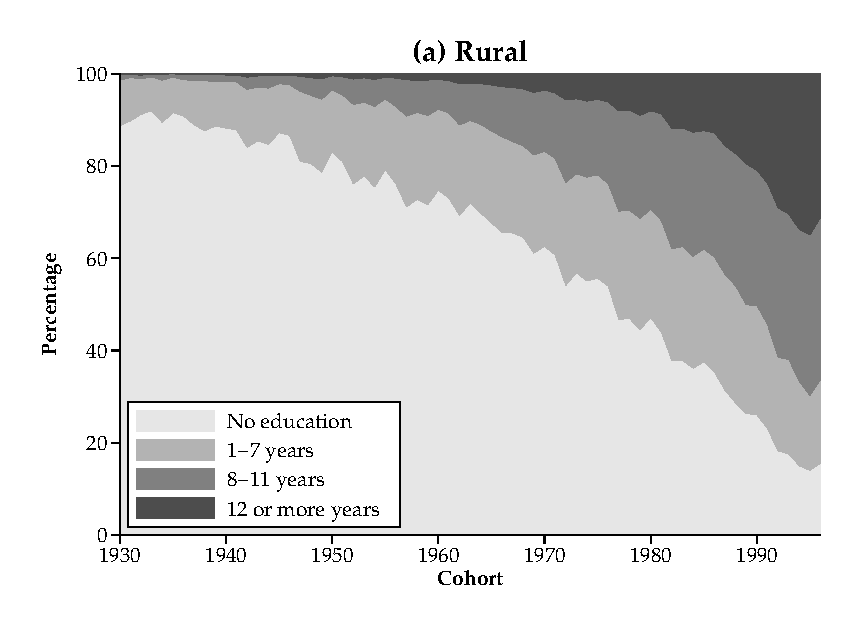
\includegraphics[width=\textwidth]{educ_over_time_rural}
    \end{minipage}
} 
\subfloat[Urban]{
    \begin{minipage}{0.49\textwidth}
        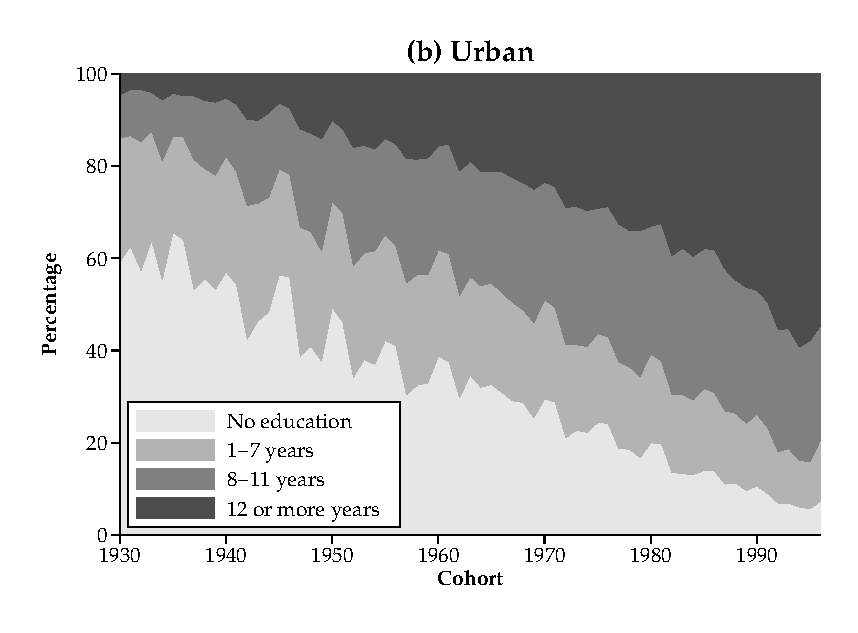
\includegraphics[width=\textwidth]{educ_over_time_urban} 
    \end{minipage}
}
\caption{Distribution of education by cohort for women 20 years or older at survey}
\label{fig:education_over_time}
\end{figure}



Families in urban areas are likely to have fewer children and higher rates of sex 
selection and, therefore, increasingly longer birth intervals over time compared to
rural families.
With the costs of children higher in urban than in rural areas both because of the
lower opportunities for productive work of children and the higher cost of consumption
related to children, fertility is expected to be lower in urban than in rural areas.
Furthermore, access to health care and generally a healthier environment because of,
for example, cleaner water means that urban parents can have fewer children and invest
more in each than in rural areas.%
\footnote{
However, holding parental education constant, there is evidence that children in
Indian slums do worse than they would have in rural areas \citep{Portner2018a}.
}
However, the better access to health care also means that there is easier access to
sex selection and the generally higher income of urban households makes it more
affordable.
[differences in birth intervals without sex selection?]


Wages generally increase with education suggesting that higher female education
should shorten birth spacing and lower fertility, but also increase the use of sex 
selection.
However, female education undoubtedly represents more than the value of women's time.
Two examples are the productions of child health and offspring human capital.
[something on norms?]

First, children of more educated women tend to have better health outcomes and lower 
mortality than less educated women, either from higher income or better health knowledge 
\citep{Rosenzweig1982a,Kovsted2002,Whitworth2002,Maitra2008}.
Lower expected mortality means that fewer births are required to reach a desired
number of surviving children.
Similarly, although short birth spacing generally leads to worse health outcomes, 
the more educated the mother, the more muted this relationship is, which, at least partly,
removes the health outcome incentive for longer birth spacing
\citep{Whitworth2002,Conde-Agudelo2012,Molitoris2019}.

Second, better-educated women are more efficient at producing child human capital 
\citep{Behrman1999}.
[need something on son preference? Maybe simply use increasing returns to male education]
Hence, families that value sons' education more will tend to both demand better-educated
women as mothers and have fewer children because both allow for higher quality boys.
With the increasing return to male education that India has experienced, this imply
an increased demand for better-educated women combined with lower fertility, and an 
increased use of sex selection when available.
In this case, the associations between higher female education, lower fertility, and more
sex selection are not a causal effect driven by higher wages but instead the result of the 
increased return to male education. 

Even as the level of female education has increased, the female labor force 
participation in both urban and rural areas has stagnated or decreased
\citep{Klasen2015,Fletcher2017,Afridi2018,Bhargava2018,Chatterjee2018,Bhargava2019}.
India's female labor force participation is now one of the lowest in the world  
and does not yet show any signs of increasing \citep{Klasen2015,Chatterjee2018}.
In line with previous research, the NFHS data show a U-shaped relationship between 
education and working for married women, with the highest percentage working being women 
with either no education or 12 or more years and the lowest being women with 8--11 years 
of education.%
\footnote{
See appendix Figures \ref{fig:work_by_survey} through \ref{fig:work_family_by_survey}. 
}

The low and declining female labor force participation, especially for younger women, 
suggests that families face little incentive to space children more closely 
together for economic reasons.
One explanation is that household income has increased so substantially that the income 
effect dominates any substitution effect.
Two findings speak to this effect.
First, although real wages for both men and women have almost doubled between 1987 and 
2011, the mean male wage is still close to 70\% higher than the female wage 
\citep{Klasen2015,Bhargava2018}.
Second, women’s labor supply appears to be more negatively elastic to husbands' 
wages than positively elastic to their own wages \citep{Bhargava2018}.

% Sanskritization

The increases in female educational attainment imply that access to education has 
expanded beyond the higher castes. 
One possible effect of the associated change in the composition of better-educated women 
is that this group's behavior would change.
However, ``Sanskritization'' implies that as lower-castes females gain access to 
education and their husbands' income increases, they adopt higher-caste 
norms such as stronger son preference and a retraction from the formal labor 
market \citep{Srinivas1956,Chen1995,Abraham2013,Chatterjee2018}.
The low and declining female labor force participation suggests that this process still operates.

% Summary / hypotheses

In summary, with substantial increases in husbands' income and a declining female labor 
force participation, I expect a push toward longer birth spacing over time, independent
of education levels, based on the income effects and the effects of spacing
on child outcomes.
Furthermore, I expect birth spacing to increase the most among the better educated 
because their household income increases the most---even with declining female labor 
participation---and because of their use of sex selection.
Even with the substantial increase in the number of better-educated women, 
"Sanskritization" implies that the changing composition will not substantially change 
the use of sex selection.






